%------------------------------------------------------------------------------
%Description       : DDMoRe WP7.2.1 Functional Specification for the Model
%                                   Repository Infrastructure - Proposed Design 
%Author            : Mihai Glonț <mglont@ebi.ac.uk>
%Organization      : EMBL-EBI
%                    Wellcome Trust Genome Campus
%                    Hinxton
%                    Cambridge
%                    United Kingdom
%------------------------------------------------------------------------------
\section{Direct interaction with the \ddmore Model Repository}
\label{directInteraction}
Having defined the context and the needs of the \ddmore Model Repository, we now proceed to describe the capabilities and behaviour of the envisaged solution. We present a high-level view of the features that will be available. A comprehensive list of scenarios illustrate how each of the stakeholders from Section~\ref{users} interacts with the system. Each such interaction is called a \gls{usecase}, while the user performing it is known as an \gls{actor}. The use cases listed in Figure~\ref{fig:useCases} only consider the main actors that are involved, hence Administrators are not mentioned in any model-related use cases, in spite of the fact that they do have the authority required to perform any action.

\begin{figure}[htb]
\centering
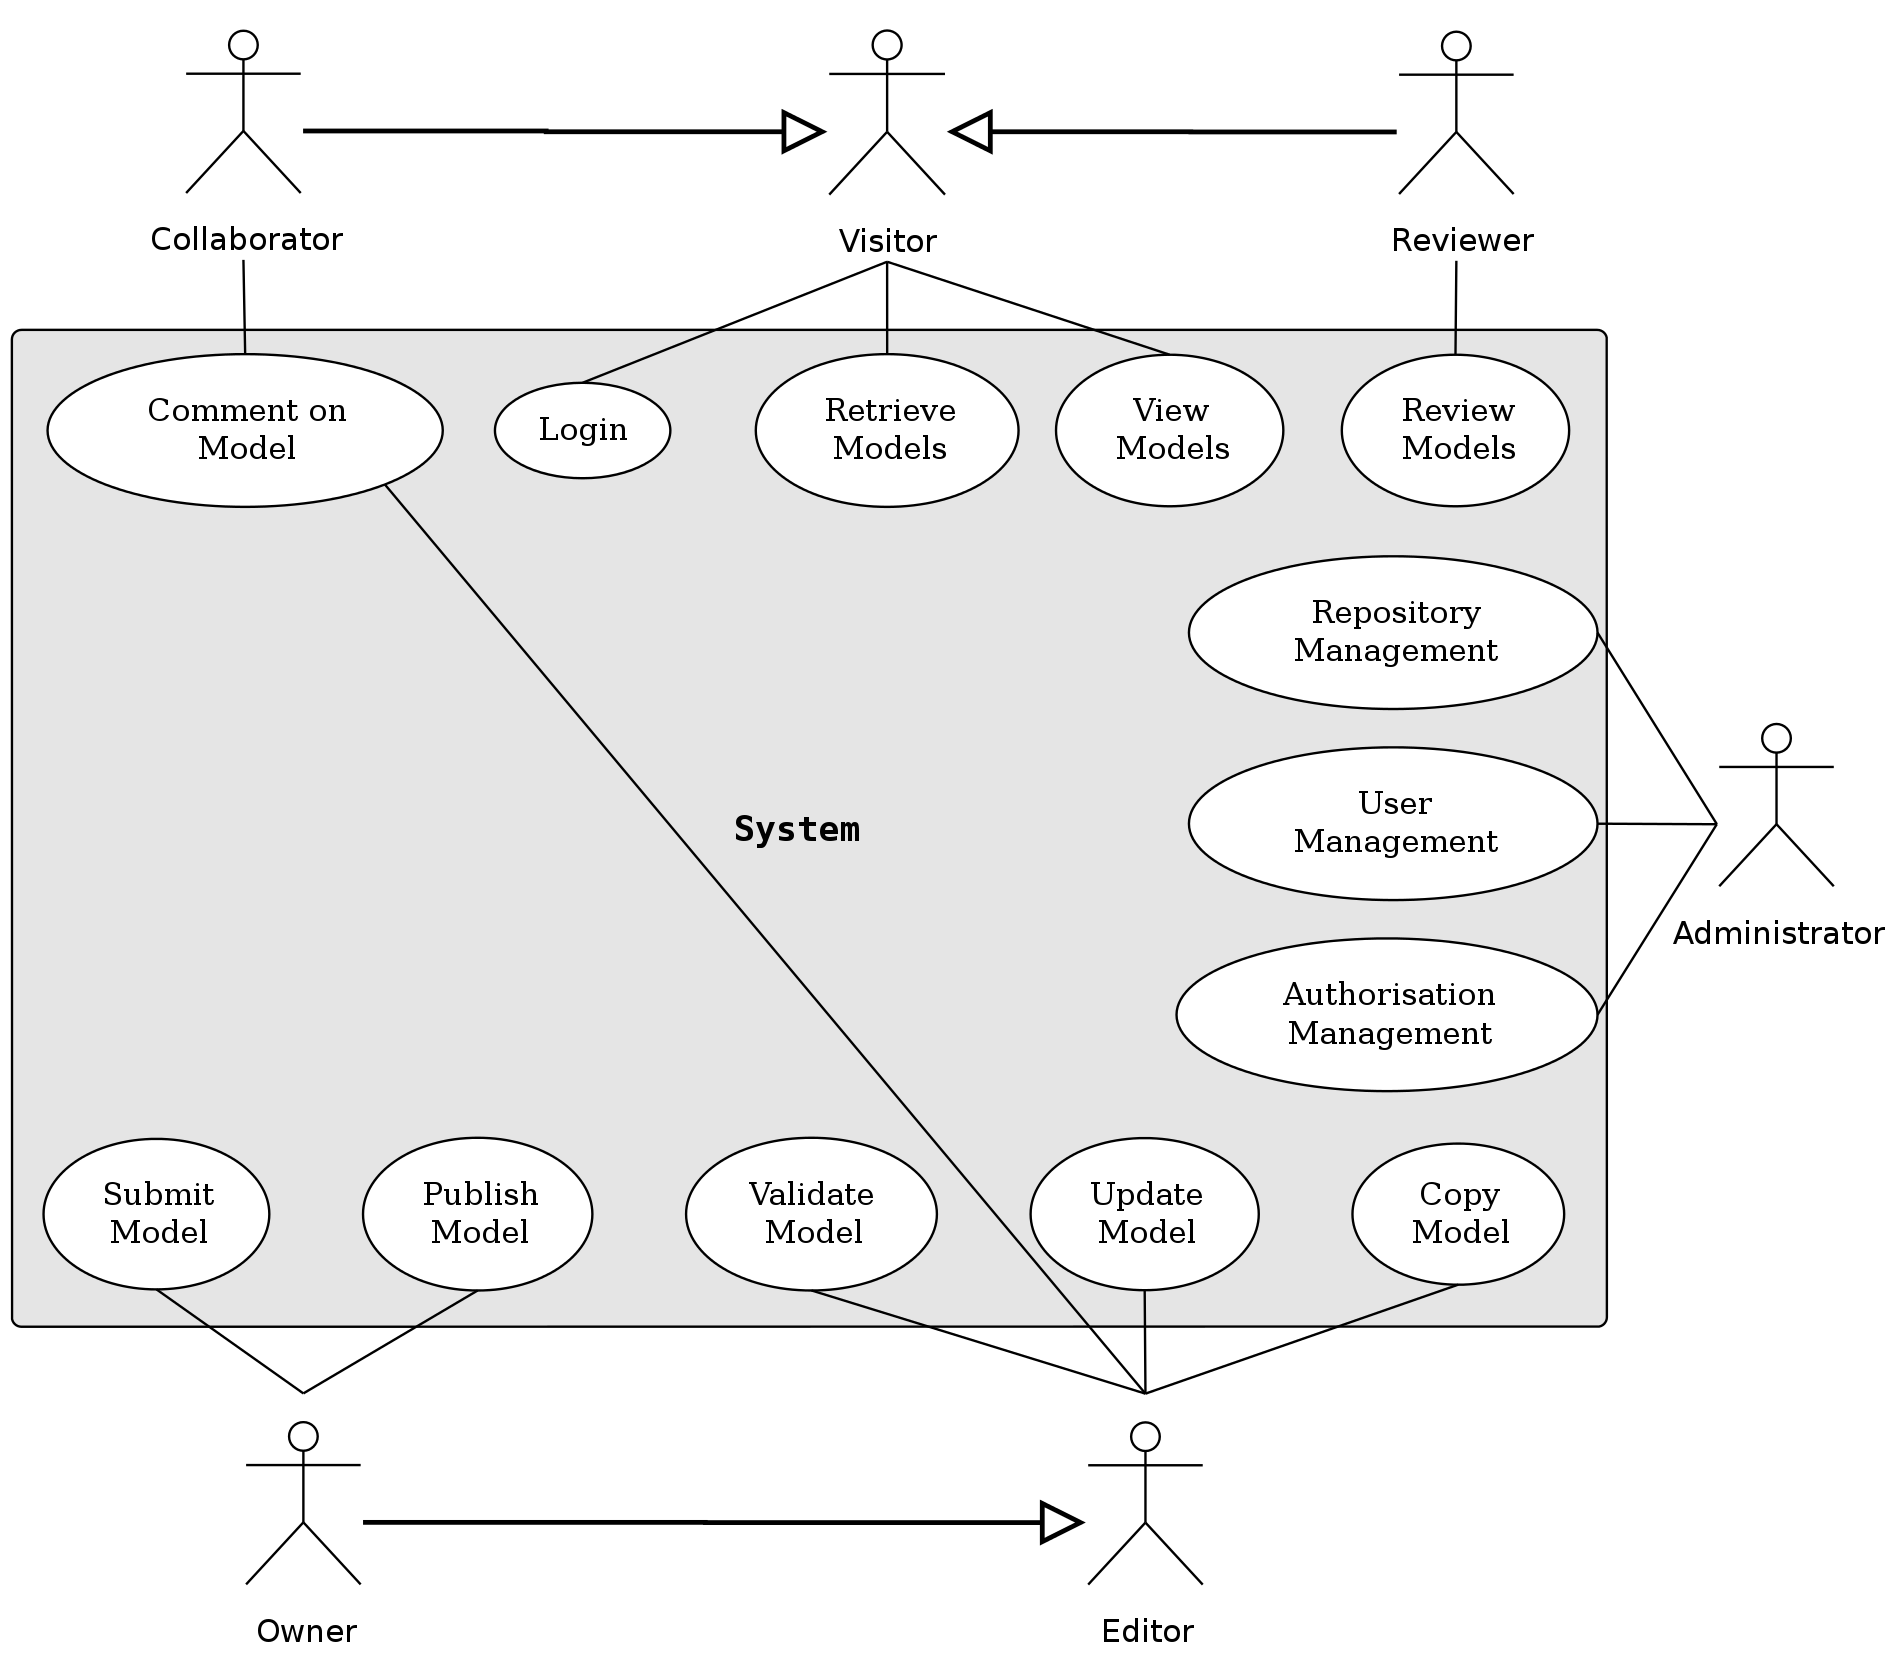
\includegraphics{img/UseCases}
\caption{Diagrammatic representation of the system's scope.}
\label{fig:useCases}
\end{figure}

\subsection{Initial considerations}
\subsubsection{User profiles}
\label{userProfiles}
The scenarios listed below are illustrated from the perspective of the following users:
\begin{description}
    \item[Joe] -- a scientist interested in preclinical models of prostate cancer.
    \item[Sam] -- an Administrator of BestModels, a private instance of the \ddmore Model Repository used internally at BestMeds PLC, a large pharmaceutical company.
    \item[Hannah] -- a highly experienced PKPD modeller working at BestMeds PLC that has contributed to the development of many models which are deposited in BestModels.
    \item[Julia, Dominic, and Sue] -- young, but very promising modellers that have recently joined BestMeds PLC.
\end{description}

\subsubsection{MML Structure}
At the time of this writing, the specification of MML is under development. Given that features such as model submission, template creation, publication, search, or model display are dependent on the MML structure, there is a limited amount of information we can include about them at this stage. The discussion of these sections will be expanded once MML becomes publicly available.

\subsection{Model development}

\subsubsection{Submitting a model}
%\idea{public instance: no authentication will be required. \textbf{ToDo: Write story about Joe that is studying the role of a particular type of flavonoid called Quercitin in inhibiting carcinogenesis.}}
Submitting a model to the public instance of the \ddmore Model Repository will not require the submitter to create an account or log-in, and will make the modelpublicly-available. The process depends very much on the structure of the MML, and the kind of model that is being submitted. However, we should start by collecting information about its creators. Then, the Repository should validate the model and report any issues back to the submitter as grounds for rejecting the model. Once the model is deemed fit, any cross-references contained within the model should be digested, so that we can enhance the understanding of the model's context. Then, the Repository will store the model and assign it a perennial identifier. We should also display a confirmation page right before we start processing the new model so that the submitter is offered a chance to address incorrect details.

Let us imagine Julie wants to submit her latest work to BestModels. She logs in by typing her username and password and clicking on the \textsc{Login} button. She is then shown her user homepage, containing a list of models which she has developed. If the model she has been developing is not already in BestMeds, Julie selects the \textsc{Submit new model} action which is displayed above her list of models. Alternatively, she simply selects the model that she has been working on. This brings a new page that describes that model in more detail, including its versions.  

Since Julie has write-access rights to this model, she is able to click the \textsc{Submit new version} button from the list of actions that are available to her. Had this not been the case, Julie would have not been able to update the model. The Model Repository pre-populates fields such as model name, model identifier or model authors. Then, Julie uploads the new version of the model which is processed by BestModels. Next, we display the list of collaborators that will have access to this version based on the previous one, giving Julie the chance to update it. Once she confirms who will be able to access this version, BestModels displays a summary of the model version that is about to be submitted, giving Julie the choice to \textsc{Finish}, or to go \textsc{Back} and make any amendments. Julie clicks \textsc{Finish} causing the new model version to be processed. Upon completion, BestModels reports whether the submission was successful or not.

\begin{techNote}
A Strategy pattern should be used, whereby each kind of model that is handled by that instance of the Repository corresponds to a class in charge of the submission algorithm; there needs to be a \texttt{SubmissionStrategy} interface containing a \texttt{submit} method. The Repository will have a plugin dedicated to each kind of model it supports. These plugins will implement the \texttt{SubmissionStrategy}. In addition, a \texttt{SubmissionManager} maintains a reference to a \texttt{SubmissionStrategy} object and is in charge of forwarding the submission responsibility to the correct plugin.
\end{techNote}

\subsubsection{Model Templates}
%The process of generating a model from an existing one largely depends on the structure of the MML. 

The typical work flow starts with a user viewing a model revision stored in the \ddmore Model Repository. The user selects the components of the model that they wish to include in the new model. What constitutes a model component is MML-dependent, but it might include, for instance, the structural model or any subset of its elements, simulation results, final parameters or clinical data. The Repository will assemble the selected components into a valid MML encoding, and will allow the user to download it. 

\subsubsection{Deleting models}
The user that has write-access rights to a model may delete a version of it.  This is achieved by logging in, clicking on the model they are interested in, in order to view it in more detail, then choosing the \textsc{Delete} button next to the version in question. The Repository then asks if there is a replacement. The user has the choice to provide a link to a new version that (s)he can access, or not provide a replacement. The Repository will trigger an error message if the user cannot access the replacing version. The user clicks on the \textsc{Confirm deletion} button and receives a visual confirmation of status of the removal. 

%Also, the user must be able to specify replacements for his(her) deleted versions at a later stage, so we need the concept of a Bin or Archive. 
As far as other users are concerned, when they access the deleted version they will still see its contents, but a clearly-visible message will inform them that it is obsolete.

\subsubsection{Subscribing to model changes}

\begin{techNote}
we need a messaging system for this -- there is no efficient/scalable alternative. we store three kinds of notifications: 
\begin{itemize}
\item model-related -- new models, updates to the access rights of existing models
\item revision-related -- new revisions, deleted revisions, updated permissions, published revisions
\item comment-related -- new comments on existing revisions.
\end{itemize}
\textbf{Note: reviews are outside the scope of the notification system.}

Each \texttt{Model}, \texttt{Revision} and \texttt{Comment} therefore need to extend \href{http://docs.oracle.com/javase/6/docs/api/java/util/Observable.html}{\texttt{java.util.Observable}}. A \texttt{NotificationObserver} implementing the \href{http://docs.oracle.com/javase/6/docs/api/java/util/Observer.html}{\texttt{java.util.Observer}} interface will aggregate every change to every model, version, or comment. This object will be a \emph{Topic Publisher} in \emph{ActiveMQ} parlance -- a producer of messages. We will dedicate a \emph{Virtual Topic} to every user that expects notifications. At the other end, there will be a \emph{Consumer} in charge of forwarding the updates to the user. 
%We will have one queue per user that has subscribed to notifications about model updates. \textbf{translate into "english" that binding keys govern the routing process and that when a user clicks on "subscribe", we create a queue that captures all messages that start with modelID, regardless of what follows it.} The structure of the message needs to be agreed upon. We could use \texttt{source.action}
\end{techNote}

\subsubsection{Publishing a model}
\label{publish}
This feature only applies to private instances of the \ddmore Model Repository. 

Let us assume that Sue has been working hard on a model and she is very pleased with it, especially since it underwent a quality-control check, and the reviewer asked Sue to share it with everyone else, so that all modellers can learn from it. 

To achieve this, Sue logs in to BestModels and sees the homepage containing her models. As before she navigates to the display page for her model, and clicks on the \textsc{Publish} button next to the version that she wishes to publish. She would not be able to publish the model if she was not its owner. Sue confirms that she wishes to make this version available to all users. Since BestModels is configured to authenticate users before displaying a model, regardless of whether it is private or public, Sue has effectively shared the model with every person that has an account on BestModels. If BestMeds provided free access to its public models, then the visibility of Sue's model would have been much larger.

%for private instances, as a model owner, you go to "My Models", which is on the homepage of every authenticated modeller. 
%Click on the model you're interested in, which renders it in detail. You go to the \textsc{Revisions} section and select 
%the one(s) that you are interested in. Then you click publish. The system indexes the changes (\textbf{todo: decide when and how}) 
%and outputs a confirmation message if the action was performed successfully. 
%If it goes belly-up, then we could be in a lot of trouble, as data integrity could be compromised. 
%there will be no way of reverting the model from the VCS, not to mention the DB. The horror


\subsection{Model browsing, searching and retrieving}

\subsubsection{Browsing models}
The \ddmore Model Repository will need to present a potentially-long list of models of various types in a user-friendly manner. Pagination and facets should be considered. A more detailed discussion of this topic will be provided once the structure and the scope of MML becomes clear.

\subsubsection{Model display}
The user interface to show models will consist of the following blocks:
\begin{itemize}
\item model
\item metadata -- includes development history, creation/modification dates, authorship etcetera on the one hand, and clerical data on the other.
\item actions -- lists all actions that are available to the user, for instance parameter estimation, simulation, or download.
\end{itemize}

The display will depend on the model type and may vary from one instance of the Model Repository to another.

\subsubsection{Model search}
The \ddmore Model Repository supports the field of drug development by allowing stakeholders to find models that are relevant for their research. The search mechanism will include all models that are available to the user performing the search: this means that in private instances, the results will contain not just publicly-available models, but also private models that the user has access to.

%\idea{story about Joe, the Visitor of the public instance that surveys PK models of flavonoids and their influence on the human body. He performs a search using the term flavonoids.}

% As such, Joe, a Visitor of the DDMoRe Model Repository would have free access to the published models that are stored in that instance without needing to register or sign in. Joe would also be able to 
%\subsubsection{Advanced search criteria}
%% including all revisions of a model in the search poses a problem at the annotation level: 
%% you end up with a lot of duplicated triples 
%% not tracking the revision of the model from which we are generating RDF impacts the relevance of the search results, as you might get a model which at some point was semantically-meaningful to the search, but you don't know at which revision it became relevant, or at which revision it stopped being being relevant to the search query.
%% it may also be difficult to delete the triples generated by a model, as it may break associations/links.
%%
%\begin{techNote}
%we need to switch between searching the latest version of each model and every single accessible version. the easiest way to implement this would be to maintain two separate indexes, one for each type of search, but this will impact the time to generate and maintain them. 
%\end{techNote}

%\idea{include a scenario where private models are included in the search as well.}


\subsection{Model quality assurance}

\subsubsection{Model review}
When we discussed \nameref{publish}, we mentioned that Sue's model underwent a review process. In this section we describe what this entails.
For Sue, the model owner, she got her version of the model in a state she is reasonably happy with, that contains valid MML and that has been executed successfully. In order to request a review, Sue logs in, navigates to the page displaying her model in detail, as described previously and  she clicks the \textsc{Submit for review} button next to the version in question. Then, Sue selects Hannah as her reviewer and clicks the  \textsc{Finish} button. Now, the model appears in the "Models under review" section of her homepage.

Hannah is now able to see Sue's model on her homepage, in the "Models I review" section. Hannah selects the model, so that she can see it in detail, and clicks on the only action that is available: \textsc{Review}. After evaluating the model in question, Hannah rates its quality using one of the scores below and [optionally] offers suggestions to Sue in the form of textual comments. Being impressed, Hannah adds a note asking Sue to publish the model, then clicks \textsc{Submit review}. Sue is now able to see that feedback is available for her model. 

It is important to mention that once a model version enters the review process, it cannot be published until it is deemed fit by the reviewer.

\begin{techNote}
The quality of the model will be evaluated using one of the following grades, listed in descending order:
\begin{itemize}
\item Pass
\item Pass with minor changes -- minimum score required for a model version to be publishable
\item Major Changes required -- this will force the authors of the model to develop a revised version of it and will by default grant the reviewer access to the updated version. 
\item Reject
\end{itemize}
If the model gets published, reviews should not be displayed. 
\end{techNote}

\begin{techNote}
Developers should decide, based on user feedback, the means to select users. One idea is to provide a text box with auto-completion functionality. Another one would be to use the jQuery UI Selectable widget in conjunction with an unordered list HTML element. Either way, check boxes should be avoided. Within an instance of the Model Repository, there will be a single method to select users, in order to aid consistency.
\end{techNote}

\subsubsection{Model validation}
This will be performed automatically by the Repository whenever a new model or version of a model is submitted. Users will also be able to do so by clicking on the \textsc{Validate} button next to each revision. A model will not be accepted in the Repository if it does not pass validation. 

\begin{techNote}
The implementation for this feature is as simple as loading the model into the API developed by WP2.3, then calling its \texttt{validate} method; if validation failed, we rely on the API to provide the cause. We will then display those error messages back to the user.
\end{techNote}

\subsection{Repository management} 

\subsubsection{User registration}
The Administrator chooses whether new users can register themselves or not. The registration process will record \textbf{at least} the following user details:
\begin{itemize}
\item First Name
\item Last Name
\item username
\item password
\item email
\end{itemize}


\begin{techNote}
In order to prevent robots from registering, a CAPTCHA code should also be included. LDAP support will be provided, minimising the number of username and password combinations users need to remember. 
\end{techNote}


\subsubsection{Suspending accounts}
Due to irreconcilable differences with her manager, today is Hannah's last day at the office. Sam, therefore needs to revoke her access to the Repository from now onwards, so that she cannot steal company secrets. 

To achieve this, Sam logs in and navigates to the User Management section. Here he can see a list of all active and inactive users of the Repository displayed as a paginated table. From the list of actions that are displayed along each record, Sam selects \textsc{Disable account}, thus suspending Hannah's account. From now on, any attempt to log in using her credentials will result in an error message that will inform the user about the ban. The account will remain in the system for security purposes, hence Sam will be able to re-enable it, if need be.

\subsubsection{Creating user lists}
BestMeds PLC  wants to enhance the collaboration between the teams of modellers within the organisation. As such, Sam has been tasked to facilitate sharing a model with multiple people.

Consequently, he logs in to BestModels and navigates to the Team Management section. This contains a list of the names of all existing teams along with \textsc{Delete} and \textsc{View} buttons. Above and below this list there is a \textsc{Create team} button. By clicking on this button, Sam is taken to the page to create a new team. He types the name of the team --- \emph{PKPD-Modelling} --- and clicks \textsc{Confirm}. The system ensures that the team name only contains letters, digits, dashes (--) and underscores (\_) and then creates the new team. If Sam had named the team \emph{PKPD-Modelling-Rockstars!}, the Repository would have informed Sam about the problematic exclamation mark.
\begin{techNote}
Since there is a many-to-many relationship between users and teams/lists, we need three tables: 
\begin{itemize}
\item users - has userID
\item teams - has teamID
\item teamRosters - links userID with TeamID. 
\end{itemize}

When a new member is added to a team, we create a new row in TeamRosters. 

When we delete a team member, we remove the corresponding association from TeamRosters.

It must be possible to share a model with a whole team - think Composite pattern for users and teams.

When we work out whether a model is accessible or not to a user, we need to go through the lists that he has access to.
\end{techNote}

\subsubsection{Deleting user lists}
\idea{this action will cause users to lose access to certain models. discuss whether this is problematic.}

Sam logs in, goes to Team Management. Clicks on the \textsc{Delete} button next to the team he wishes to delete. He is advised that this will prevent members to access the models shared with the list and asked to confirm that he wishes to delete the list in question, being given the choice to \textsc{Confirm} or \textsc{Cancel}. Clicking on the latter leaves the list as it is. By choosing the former, the list is removed and every user that gained access to models through the team will no longer be able to view them.

\subsubsection{Adding a user to a list}
As before, Sam visits the Team Management section of BestModels and selects the PKPD-Modelling team to view its roster. Since it is empty, the only action that is available is to \textsc{Add new members}, which brings a page where Sam can select the users he is interested in, as described in the technical note from the \nameref{review} section --- in this case, Julia, Hannah and Dominic. He then clicks the \textsc{Add} button. The Repository ensures that the user accounts in question exist and only then associates them to the designated team. Users can be part of multiple lists.


\subsubsection{Removing a user from a list}
\idea{discuss whether this is problematic.}

Today Sam received an email informing him that, for productivity reasons, Dominic has been assigned to a new project and that he should be removed from the team he is on. Sam therefore navigates to the User Management section of the Model Repository and selects the \textsc{View Teams} button from the list of actions that are available for Dominic's account. This brings up a page that displays all the lists that Dominic is part of and, alongside their name, there is a \textsc{Delete} button which eliminates Dominic from that list. Sam is asked, through a dialog box, to acknowledge that this action may cause Dominic to lose access to certain models by clicking on the \textsc{Confirm} button. Sam also has the option to \textsc{Cancel} this action, but since he performed it intentionally on this particular occasion, he chooses \textsc{Confirm}.

\subsubsection{Managing model ownership}
Given Hannah's departure, Sam wishes to re-assign her models to one of her close collaborators, Julia. From the same list of actions that are displayed along each user, Sam chooses \textsc{view models}, which brings up a table of every model, public or private, to which Hannah has contributed, excluding those that have been deleted. From there, Sam can quickly select the all the models developed by Hannah and clicks on the \textsc{Change role} button. This pops up a dialogue box with two buttons - \textsc{Confirm} and \textsc{Cancel}, where Sam types Julia's username and clicks \textsc{Confirm}. The system employs auto-completion using the names and usernames of the people registered in the Repository, and it will only enable the confirmation button once it has verified that Julia's account is active. If no suitable user account is found, then a meaningful error message is displayed below the text box, describing the reason why no account matched Sam's input. 

\begin{techNote}
The models should be listed in a table. The following headings could be used
\begin{itemize}
\item accession number -- a unique, perennial identifier for the model. Clicking on a it would then take Sam to the page dedicated to that particular model. 
\item model name -- the name of the model, as specified by its creator.
\item summary -- a brief description of the model.
\item role -- the role (Section ~\ref{users}) of the user -- in our case Hannah. 
\item visibility -- whether the model is public or private. 
\end{itemize}
The selection will be made  using the jQuery UI Selectable widget with the appropriate CSS selector filter. In addition, above and below the table of models there should be \textsc{Select all} and \textsc{Deselect all} buttons along with the commands \textsc{Re-assign models} and \textsc{Change role}.
\end{techNote}

%\subsection{Proposed work flows}
%\label{workFlows}
%\idea{Scenarios/Stories go here, along with UML Activity and Sequence diagrams.\textbf{Do we need these?}}

%\subsection{Mock-ups}
%\label{mockUps}
%\idea{General UXD comments behind the look and feel of the pages. Actual mock-ups should be in the appendix. Landscape page format might be required for this part.
%\textbf{TODO: is this really necessary?}
%}
